
% \begin{wrapfigure}{rt}{3.2in} \centering
%    {\setlength{\unitlength}{1.0in} \begin{picture}(3.000,1.900)(0.05,.14)
%      \put(0,0.24){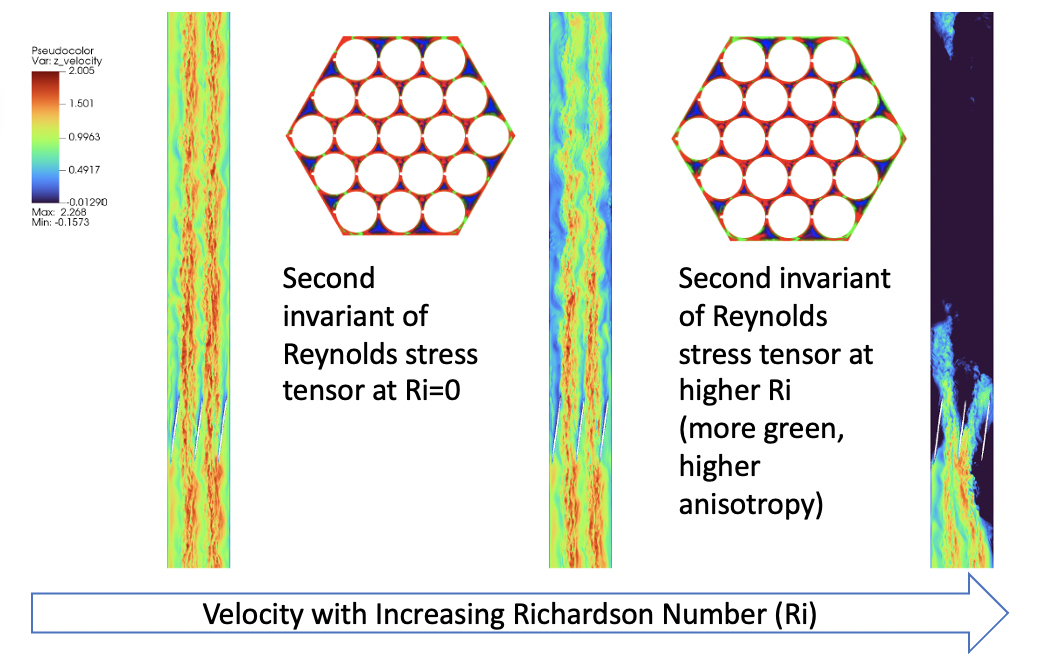
\includegraphics[scale=0.43]{figs/challenge.png}}
%    \end{picture}}
%    \caption{
% Velocity distribution in wire-wrapper assembly as a function of
%     the Richardson number at low flow conditions. \label{fig:cha1}}
% \end{wrapfigure}

\begin{figure}[t!] \centering
    {\setlength{\unitlength}{1.0in} \begin{picture}(6.5,2.000)(0.0,0)
      \put(0.0,0.10){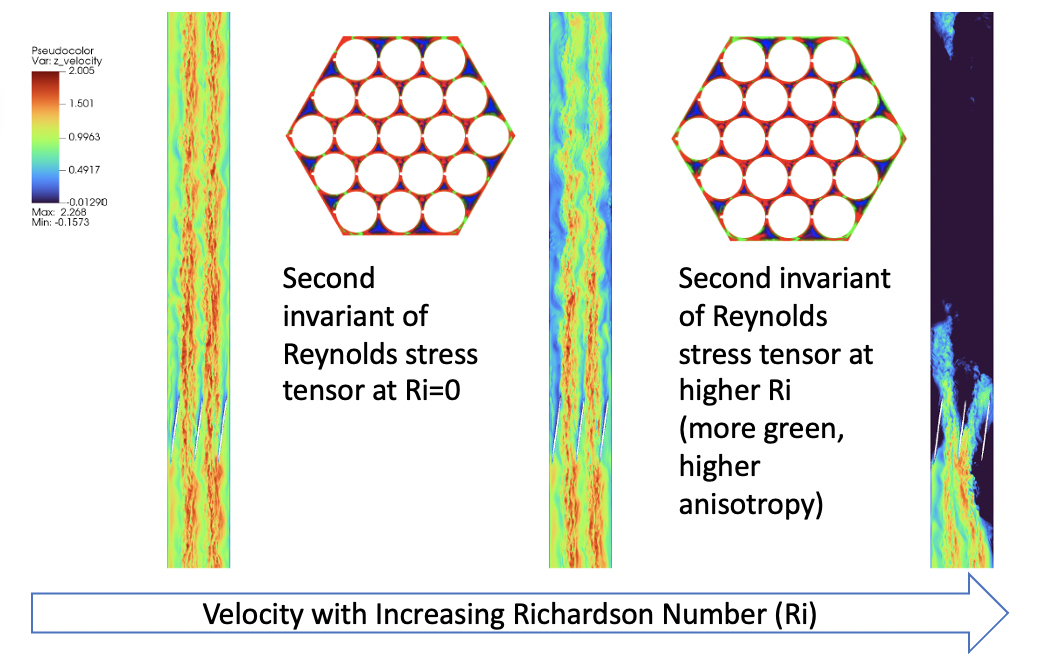
\includegraphics[scale=0.38]{figs/challenge.png}}
      \put(3.4,0.00){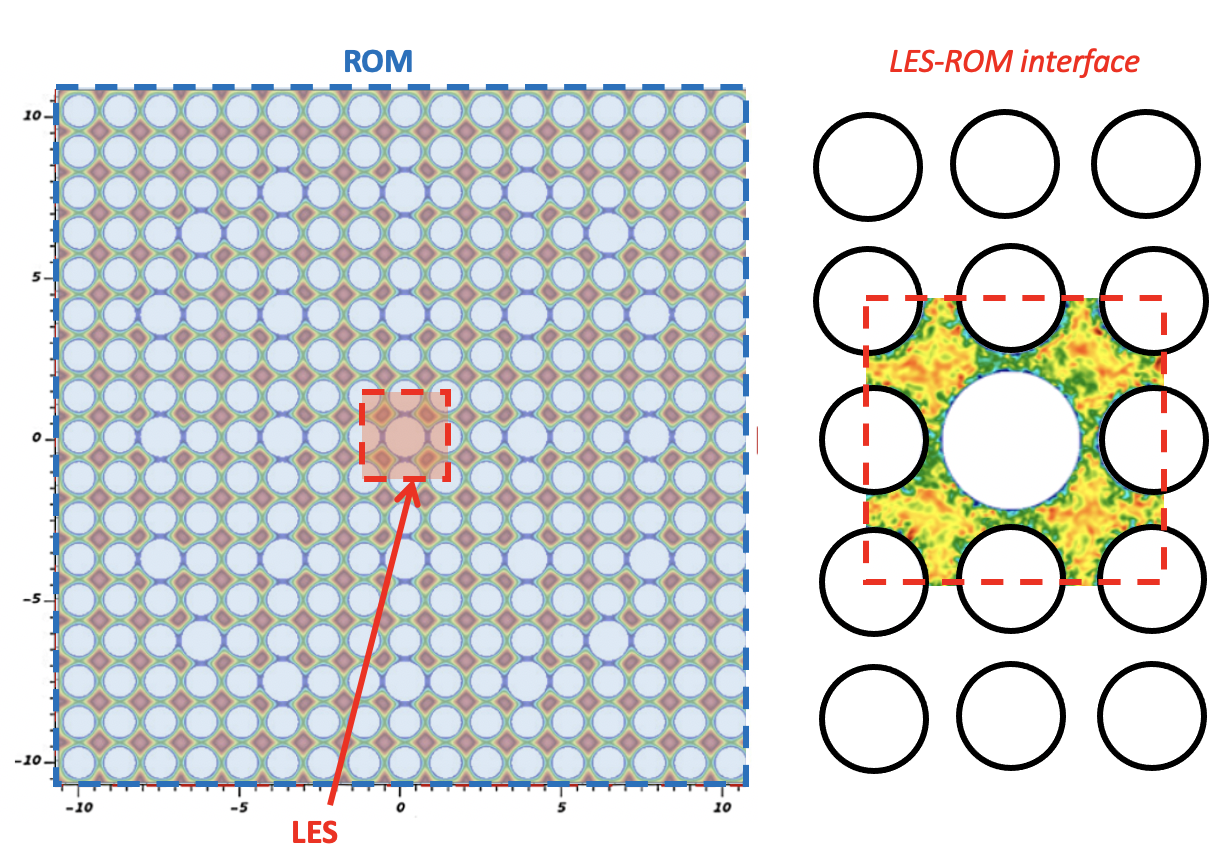
\includegraphics[height=2.0in]{figs/lesrom.png}}
    \end{picture}}
    \caption{ \label{fig:cha1}
     (left) Velocity distribution in wire-wrapper assembly as a function of
            the Richardson number at low flow conditions.
     (right) Example of LES-ROM coupling. \\[-3ex]
}
\end{figure}

\noindent \textbf{Challenge Problem.} (Tasks 1 and 3.)
We focus first on mixed convection within fuel assemblies. Fluid flow and heat removal through fuel, shield and reflector assemblies  can
have major impacts on operation and safety for Sodium Fast Reactors (SFRs).
This type of reactor is of great interest in the United States due to the
planned  deployment of Terrapower's Natrium concept funded partially through
the Advanced Reactor Demonstration program (ARDP). These assemblies are formed
by bundles from 19 to 217 pins, with a wire wrapped around each pin to maintain
the rods in place.

During transients, these assemblies are characterized by a range of conditions
that result from reduced flow rates and from large-scale organized flow
patterns, including potential intra-assembly buoyancy-driven circulation. This
in turn affects the temperature of the ducts and the overall thermo-mechanical
response of the core, which is a crucial reactivity feedback mechanism.

We note these low flow cases can provide challenges for experiments due to
complications in measuring the flow rates and temperatures with high accuracy
in different areas. This consequently also raises the uncertainty of many
modeling approaches for these phenomena, where existing correlations and
sub-channel methods fail. An example of the complex range of flow patterns in
provided in Fig. \ref{fig:cha1}(left), which shows a transition from steady forced
convection to mixed convection.  Massive circulations are introduced: in a
realistic transient the bundle will encounter the full range of conditions. We
ultimately seek methods that can provide accurate and \textit{predictive}
results. After success in this challenge problem we will tackle thermal striping and thermal stratification as stretch goals.
